%!TEX TS-program = pdflatex
%!TEX TS-options = -shell-escape
%!TEX root = trajectory-grouping.tex
% -- Author: Jannes Bantje, j.bantje@wwu.de
\documentclass[a4paper,index=totoc,toc=bibliography,fontsize=11pt,DIV=13,headinclude,BCOR=5mm,cleardoublepage=empty,ngerman,draft]{scrreprt}
\usepackage{scrpage2} % wie fancyhdr, nur optimiert auf KOMA-Skript, leicht andere Syntax
\usepackage{etoolbox,letltxmacro} % zum Programmieren
\usepackage[final]{graphicx}
\robustify\rotatebox

% -- Farben
\usepackage[x11names]{xcolor}
\definecolor{dark_gray}{gray}{0.45}
\definecolor{light_gray}{gray}{0.6}
\definecolor{fb10_blue}{cmyk}{0.8,0.4,0.13,0.07}

\usepackage[utf8]{inputenc}
\usepackage[T1]{fontenc}
\usepackage{mathtools} % beinhaltet amsmath
\mathtoolsset{centercolon,showmanualtags}
\newtagform{brackets}{[}{]}
\usetagform{brackets}
\usepackage{fix-cm}
\usepackage[bbgreekl]{mathbbol}
\usepackage{amssymb} % zusätzliche Symbole
\usepackage{nicefrac} % schräge Brüche
\usepackage{faktor}
\newcommand{\Faktor}[1]{\faktor[\textstyle]{#1}}
\usepackage{xfrac}
\usepackage{cancel}
\usepackage{mathdots} % Verbesserung von Punkten wie zB \ldots
\usepackage[bb=px]{mathalfa}
\usepackage{centernot}

\usepackage{silence}
\WarningFilter{latexfont}{Size substitutions with differences}
\WarningFilter{latexfont}{Font shape `U/bbold/m/n' in size}

%!TEX root = trajectory-grouping.tex

% -- Zum Finetuning von Befehlen
\makeatletter
\newcommand{\raisemath}[1]{\mathpalette{\raisem@th{#1}}}
\newcommand{\raisem@th}[3]{\raisebox{#1}{$#2#3$}}
\makeatother

% -- Box mit vorgegebener minimaler Länge
\DeclareRobustCommand{\minwidthbox}[2]{%
  \ifmmode
    \expandafter\mathmakebox
  \else
    \expandafter\makebox
  \fi
  [\ifdim#2<\width\width\else#2\fi]{#1}%
}

% -- farbiges Untersteichen im Mathe-Modus
\def\mathul#1#2{\color{#1}\underline{{\color{black}#2}}\color{black}} 


% -- besserer underbrace befehl
\newcommand{\Underbrace}[2]{{\underbrace{#1}_{#2}}}





%--Mengen
\newcommand\SetSymbol[1][]{\nonscript\:#1\vert\allowbreak\nonscript\:\mathopen{}}
\providecommand\given{} % to make it exist
\DeclarePairedDelimiterX\set[1]\{\}{\renewcommand\given{\SetSymbol[\delimsize]}#1}

% -- Betrag und Skalarprodukt
\DeclarePairedDelimiter{\abs}{\lvert}{\rvert}
\DeclarePairedDelimiterX\skal[2]{\langle}{\rangle}{#1\,,\,#2}

%--Umklammern
\DeclarePairedDelimiter\enbrace{(}{)}
\DeclarePairedDelimiter\benbrace{[}{]}
\DeclarePairedDelimiter\homo{\llbracket}{\rrbracket}
\newcommand{\ssbrace}[1]{{\scriptscriptstyle\enbrace{#1}}}

%--Norm
\DeclarePairedDelimiter\norm{\Vert}{\Vert}






% - verbessertes Integral
\newcommand{\Int}[1]{\int_{\mathrlap{#1}}\,\,}

% -- Alles spezielles aus der Differentialtopologie
\newcommand{\Tang}{\ensuremath{\mathrm{T}\mkern-0.85mu}}
\newcommand{\mathd}{\ensuremath{\mathrm{d}\mkern-0.7mu}}
\newcommand{\diff}[2]{\ensuremath{\frac{{\partial #1}}{{\partial #2}}}}
\newcommand{\diffs}[2]{\ensuremath{\partial #1/\partial #2}}
\newcommand{\diffd}[2]{\ensuremath{\frac{\mathd #1}{\mathd #2} }}
\DeclareMathOperator{\Lie}{L}
\DeclareMathOperator{\Ad}{Ad}  
\DeclareMathOperator{\ad}{ad}
\DeclareMathOperator{\Spin}{Spin}
% \DeclareMathOperator{\spin}{spin}
\newcommand{\spin}{\mathop{\mathfrak{spin}}}
\newcommand{\Ce}{\mathcal{C}}
\DeclareMathOperator{\vol}{vol}



%--Abbildungsdefinition
\newcommand{\mapdef}[5]{%
	\[
		\begin{array}{rcl}
			\textstyle #1 &\xrightarrow{\minwidthbox{#5}{2em}} & \textstyle #2 \\[0.5ex]
			\textstyle #3 &\xmapsto{\minwidthbox{\mbox{ }}{2em}} & \textstyle #4
		\end{array}
	\]
}

%--modifiziertes Stackrel
\newcommand{\StackText}[2]{\stackrel{\mbox{\scriptsize #1}}{#2}}
\newcommand{\StackTextClap}[2]{\stackrel{\mathclap{\mbox{\scriptsize #1}}}{#2}}



 % Liste mit Mathebefehlen laden

% -- TikZ-Kram
\usepackage{tikz-cd}
\usetikzlibrary{quotes,babel,arrows.meta}
\tikzset{>=Straight Barb[]}
\tikzcdset{arrow style=math font}

% -- tikz/externalize
\usetikzlibrary{external}
\tikzexternalize[prefix=Bilder/tikz/, up to date check=diff]
\tikzset{external/system call={xelatex \tikzexternalcheckshellescape %-- verwende LuaLaTeX, wegen dynamischer Speicherallokation
    -halt-on-error -interaction=batchmode -jobname "\image" "\texsource"}}
\AtBeginEnvironment{tikzcd}{\tikzexternaldisable}
\AtEndEnvironment{tikzcd}{\tikzexternalenable}
\pgfkeys{/pgf/images/include external/.code=\includegraphics{#1}}

% -- Einstellungen bezüglich Schriftart etc.
\usepackage{ccfonts}
\usepackage[semibold]{sourcesanspro}
\usepackage[semibold,scale=.95]{sourcecodepro}
\usepackage{eulervm}

% \addtokomafont{disposition}{\sffamily}

\usepackage{fontawesome}
\usepackage[final]{microtype}
\flushbottom
\KOMAoptions{DIV=last}


% -- Einstellungen bezüglich der Sprache, Silbentrennung etc.
\usepackage{babel}
% \usepackage{polyglossia}
% \setmainlanguage[spelling=new,babelshorthands=true]{german}
% \setotherlanguage[variant=british]{english}

% -- BibLaTeX 
\usepackage[%
	backend=biber,
	sortlocale=auto,
	natbib,
	hyperref,
	backref,
	style=alphabetic
	]%
{biblatex}
\renewcommand*{\mkbibnamelast}[1]{%
  \ifmknamesc{\textsc{#1}}{#1}}

\renewcommand*{\mkbibnameprefix}[1]{%
  \ifboolexpr{ test {\ifmknamesc} and test {\ifuseprefix} }
    {\textsc{#1}}
    {#1}}

\def\ifmknamesc{%
  \ifboolexpr{ test {\ifcurrentname{labelname}}
               or test {\ifcurrentname{author}}
               or ( test {\ifnameundef{author}} and test {\ifcurrentname{editor}} ) }}
\addbibresource{quellen.bib}

% -- Konfiguration von Hyperref
\usepackage[hidelinks, pdfpagelabels, bookmarksopen=true, bookmarksnumbered=true, linkcolor=black, urlcolor=SkyBlue2, plainpages=false,pagebackref, citecolor=black, hypertexnames=true, pdfauthor={Jannes Bantje}, pdfborderstyle={/S/U}, linkbordercolor=SkyBlue2, colorlinks=false,backref=false]{hyperref}
\hypersetup{final}

\usepackage[nameinlink,noabbrev]{cleveref}

% -- \url aufhübschen
\newcommand{\appendLink}[1]{#1\,\faExternalLink}
\newcommand{\hrefsym}[2]{\href{#1}{\texttt{\appendLink{#2}}}}
\renewcommand{\url}[1]{\hrefsym{#1}{\nolinkurl{#1}}}

% -- Aufzählungen, Anführungszeichen etc.
\usepackage[shortlabels,inline]{enumitem}
\setlist[itemize,1]{label=\scriptsize$\blacksquare$}
\usepackage[autostyle,german=quotes]{csquotes}


% -- Indexverarbeitung
\usepackage{makeidx}
\newcommand{\bet}[1]{\emph{#1}}
\newcommand{\Index}[1]{\bet{#1}\index{#1}}
\makeindex
% \setindexpreamble{{\noindent \itshape Die Seitenzahlen sind mit Hyperlinks zu den entsprechenden Seiten versehen, also anklickbar}\par \bigskip}
\renewcommand{\indexpagestyle}{scrheadings}

% -- Alles zum Thema Gliederung
% \usepackage{chngcntr}
% \counterwithin*{equation}{section}
\numberwithin{equation}{section}
% \setcounter{tocdepth}{3}

% -- theorem packages
\let\openbox\relax
\usepackage{amsthm}
\usepackage{thmtools,thm-restate}
\usepackage{mdframed}
\renewcommand{\listtheoremname}{Übersicht aller Aussagen}

% -- Theoreme als PDF-Lesezeichen
\usepackage{bookmark}
\bookmarksetup{open,numbered}
\makeatletter
\newcommand*{\theorembookmark}{%
  \bookmark[
    dest=\@currentHref,
    rellevel=1,
    keeplevel,
  ]{%
    \thmt@thmname\space\csname the\thmt@envname\endcsname
    \ifx\thmt@shortoptarg\@empty
    \else
      \space(\thmt@shortoptarg)%
    \fi
  }%
}   
\makeatother

% -- Definition der einzelnen Umgebungen
\declaretheoremstyle[%
	headfont=\sffamily\bfseries,
	notefont=\normalfont\sffamily,
	bodyfont=\normalfont,
	headformat=\NUMBER\ \NAME\NOTE,
	headpunct=.,
	postheadspace=1em,
	spaceabove=15pt,spacebelow=10pt,
	shaded={bgcolor=gray!20},
	% mdframed={%
	% 	backgroundcolor=gray!20,
	% 	innertopmargin=0pt,
	% 	innerleftmargin=0pt,
	% 	% roundcorner=5pt,
	% 	innerbottommargin=0pt,
	% 	splittopskip = 0pt,
	% 	% skipbelow=6pt,
	% 	% skipbelow=6pt,
	% 	topline=false,bottomline=false,leftline=false,rightline=false
	% },
	postheadhook=\theorembookmark]%
{mainstyle}
\declaretheoremstyle[%
	headfont=\sffamily\bfseries,
	notefont=\normalfont\sffamily,
	bodyfont=\normalfont,
	headformat=\NUMBER\ \NAME\NOTE,
	headpunct=.,
	postheadspace=1em,
	spaceabove=15pt,spacebelow=10pt,
	shaded={bgcolor=fb10_blue!20},
	postheadhook=\theorembookmark]%
{mainstyle_blue}
\declaretheoremstyle[%
	headfont=\sffamily\bfseries,
	notefont=\normalfont\sffamily,
	bodyfont=\normalfont,
	headformat=\NUMBER\ \NAME\NOTE,
	headpunct=.,
	postheadspace=1em,
	spaceabove=15pt,spacebelow=10pt,
	postheadhook=\theorembookmark]%
{mainstyle_unshaded}
\declaretheoremstyle[%
	headfont=\sffamily\bfseries,
	notefont=\normalfont\sffamily,
	bodyfont=\normalfont,
	headformat=\NUMBER\NAME\NOTE,
	headpunct=.,
	postheadspace=1em,
	spaceabove=15pt,spacebelow=10pt,
	% shaded={bgcolor=gray!20},
	postheadhook=\theorembookmark]%
{mainstyle_unnumbered}
\declaretheoremstyle[%
	headfont=\sffamily\bfseries,
	notefont=\normalfont\sffamily,
	bodyfont=\normalfont,
	headformat=swapnumber,
	headpunct=.,
	postheadspace=1em,
	spaceabove=15pt,spacebelow=10pt,
	shaded={bgcolor=gray!20},
	postheadhook=\theorembookmark,
	qed=\qedsymbol]%
{mainstyleB}
\declaretheorem[name=Definition,parent=section,style=mainstyle_blue]{definition}
\declaretheorem[name=Definition \& Proposition,refname=Proposition,sharenumber=definition,style=mainstyle_blue]{definitionP}
\declaretheorem[name=Definition,numbered=no,style=mainstyle_unnumbered]{definition*}
\declaretheorem[name=Theorem,sharenumber=definition,style=mainstyle]{theorem}
\declaretheorem[name=Theorem,numbered=no,style=mainstyle_unnumbered]{theorem*}
\declaretheorem[name=Proposition,sharenumber=definition,style=mainstyle,refname=Proposition]{proposition}
\declaretheorem[name=Lemma,sharenumber=definition,style=mainstyle]{lemma}
\declaretheorem[name=Satz,refname=Satz,sharenumber=definition,style=mainstyle]{satz}
\declaretheorem[name=Satz,sharenumber=definition,style=mainstyle_unshaded]{satzUnshaded}
\declaretheorem[name=Definition,sharenumber=definition,style=mainstyle_unshaded]{definitionUnshaded}
\declaretheorem[name=Satz,numbered=no,style=mainstyle_unnumbered]{satz*}
\declaretheorem[name=Korollar,sharenumber=definition,style=mainstyle]{korollar}
\declaretheorem[name=Korollar,sharenumber=definition,style=mainstyleB]{korollarB}
\declaretheorem[name=Frage,numbered=no,style=mainstyle_unnumbered]{frage}
\declaretheorem[name=Frage,sharenumber=definition,style=mainstyle_unshaded]{frageA}
\declaretheorem[name=Erinnerung,sharenumber=definition,style=mainstyle_unshaded]{erinnerungA}
\declaretheorem[name=Ausblick,sharenumber=definition,style=mainstyle_unshaded]{ausblick}
\declaretheorem[name=Konvention,sharenumber=definition,style=mainstyle]{konvention}
\declaretheorem[name=Notation,sharenumber=definition,style=mainstyle_unshaded]{notation}
\declaretheorem[name=Bemerkung,sharenumber=definition,style=mainstyle_unshaded]{bemerkung}
\declaretheorem[name=Bemerkung,numbered=no,style=mainstyle_unnumbered]{bemerkung*}
\declaretheorem[name=Beispiel,sharenumber=definition,style=mainstyle_unshaded]{beispiel}
\declaretheorem[name=Beispiel,numbered=no,style=mainstyle_unnumbered]{beispiel*}
\declaretheorem[name=Exkurs,numbered=no,style=mainstyle_unnumbered]{exkurs*}

% english versions
\declaretheorem[name=Remark,sharenumber=definition,style=mainstyle_unshaded]{remark}
\declaretheorem[name=Remark,numbered=no,style=mainstyle_unnumbered]{remark*}
\declaretheorem[name=Example,sharenumber=definition,style=mainstyle_unshaded]{example}
\declaretheorem[name=Corollary,sharenumber=definition,style=mainstyle]{corollary}

% -- Beweise
\declaretheoremstyle[headfont=\bfseries\scshape,bodyfont=\normalfont,headpunct=:,postheadspace=1em,spacebelow=12pt,spaceabove=2pt,qed=\qedsymbol]{beweise}
\declaretheoremstyle[headfont=\bfseries\scshape,bodyfont=\normalfont,headpunct=:,postheadspace=1em,spacebelow=12pt,spaceabove=2pt]{beweisskizze}
\declaretheoremstyle[headfont=\sffamily\bfseries,bodyfont=\normalfont,headpunct=:,postheadspace=1em,spacebelow=10pt,spaceabove=10pt]{bemerkungen}
\declaretheorem[name=Beweis,numbered=no,style=beweise]{beweis}
\let\proof\relax
\declaretheorem[name=Proof,numbered=no,style=beweise]{proof}
\declaretheorem[name=Sketch of Proof,numbered=no,style=beweisskizze]{sketch}

\declaretheorem[name=Übung,numbered=no,style=bemerkungen]{uebung}
\declaretheorem[name=Erinnerung,numbered=no,style=bemerkungen]{erinnerung}


% -- marginnotes package
\usepackage[fulladjust]{marginnote}
\renewcommand*{\marginfont}{\itshape \footnotesize}
\usepackage{ragged2e}
\renewcommand*{\raggedleftmarginnote}{\RaggedLeft}
\renewcommand*{\raggedrightmarginnote}{\RaggedRight}

% -- todonotes package
\usepackage[textsize=small,obeyDraft]{todonotes}
\LetLtxMacro{\oldtodo}{\todo}
\renewcommand{\todo}[2][]{\tikzexternaldisable\oldtodo[#1]{#2}\tikzexternalenable}
\LetLtxMacro{\oldmissingfigure}{\missingfigure}
\renewcommand{\missingfigure}[2][]{\tikzexternaldisable\oldmissingfigure[{#1}]{#2}\tikzexternalenable}

% -- Fußnoten anpassen
\deffootnote[1.5em]{1.5em}{1.5em}{\textsuperscript{\thefootnotemark}\ }

% -- Figures und Captions
\usepackage{wrapfig}

%--Römische Zahlen
\newcommand{\RM}[1]{\MakeUppercase{\expandafter{\romannumeral #1.\relax}}}
\robustify\RM


% -- Metadaten für die Titelei
\author{Jannes Bantje}


% -- Kopf- und Fußzeilen
\setheadsepline{1pt}[\color{light_gray}]
\pagestyle{scrheadings}
\clearscrheadfoot
\automark{section}
\lehead{
\includegraphics[height=0.6 cm,keepaspectratio]{Bilder/Logo_WWU_Muenster_light_gray.pdf}}
\lohead{\color{dark_gray}\normalfont\footnotesize\sffamily\itshape Gruppierung von Trajektorien -- Seminarvortrag von Jannes Bantje}
\rohead{
\includegraphics[height=0.6 cm,keepaspectratio]{Bilder/fb10logo_gray.pdf}}

\ofoot[{\color{dark_gray}\sffamily\LARGE \thepage}]{{\color{dark_gray}\sffamily\LARGE \thepage}} %hier wir auch der plain Stil bearbeitet!
\ifoot{ \color{dark_gray} \sffamily\small \leftmark}

% -- Inhaltsverzeichnis und weitere Pakte, die zuletzt geladen werden sollten
\usepackage[tocindentauto]{tocstyle}
\usetocstyle{KOMAlike}
\usepackage{ellipsis}



\begin{document}
\pagenumbering{Roman}

%!TEX root = trajectory-grouping.tex
\begin{titlepage}
\hspace*{0.12\textwidth}% Whitespace to the left of the title page
\rule{2pt}{\textheight}% Vertical line
\hspace*{0.05\textwidth}% Whitespace between the vertical line and title page text
\begin{minipage}[b]{0.80\textwidth}
	\raggedright
	
\includegraphics[height=1.5cm, keepaspectratio]{Bilder/Logo_WWU_Muenster.pdf} \\[2cm]
	{\Large \sffamily Ausarbeitung zum Seminarvortrag}\\[0.5cm]
	{\Huge\sffamily\bfseries Gruppierung von Trajektorien}\\[.5cm]
	{\large\sffamily basierend auf \citetitle{buchin2015} von \citeauthor{buchin2015}}\\[5cm]
	{\large \textit{Autor:}}\\[5pt]
	{\Large \textsc{Jannes Bantje}}\\[5pt] % Author name
	{\small\email{j.bantje@wwu.de}\\ Matr.\,Nr.: 395\,197}\\[2.5cm]
	
	\vspace{0.1\textheight}
	
\includegraphics[height=1cm, keepaspectratio]{Bilder/fb10logo.pdf}
	% \hfill\includegraphics[height=8cm,keepaspectratio]{Bilder/E8_graph.pdf}
\end{minipage}	


% \begin{center}
% \vspace*{10cm}
% \includegraphics[height=9cm,keepaspectratio]{Bilder/E8_graph.pdf}
% \end{center}

\end{titlepage}

\tableofcontents

\section*{Notation}
\addcontentsline{toc}{section}{Notation}
Im Verlauf dieser Arbeit gelten die folgenden Konventionen
\begin{itemize}
	\item 
\end{itemize}
Das Vorgehen richtet sich in erster Linie nach \textcite{buchin2015}.
\cleardoubleoddemptypage
\pagenumbering{arabic}
\setcounter{page}{1}
\setcounter{footnote}{0}

\chapter{Einleitung und Problemstellung} % (fold)
\label{cha:einleitung}
%!TEX root = ../trajectory-grouping.tex
Betrachtet man eine Menge von sich bewegenden Entitäten, so haben wir bereits im dritten Beitrag dieses Seminars festgestellt, dass für die Analyse solcher Daten eine Gruppierung einzelner Trajektorien äußerst nützlich ist.
In diesem Beitrag soll eine solche Gruppierung mit Methoden der Topologie erläutert werden.\todo{Kapitel aus Buch durchlesen, um Unterschiede betonen zu können}

Intuitiv soll eine Menge ausreichend vieler sich bewegender Entitäten, die sich für eine gewisse Zeit lang \enquote{zusammen bewegen}, eine Gruppe bilden.
Unsere erste Aufgabe wird es sein, diese Intuition in eine mathematische Definition zu überführen.
Diese intuitive Definition suggeriert bereits, dass dabei drei Parameter in eine Definition mit eingehen sollten:
\begin{description}
	\item[Mindestgröße] Auch wenn man prinzipiell den Fall einer einelementigen Gruppe betrachten kann, sollte eine Gruppe im Allgemeinen eine gewisse Mindestgröße haben, die sich gegebenenfalls aus dem Anwendungsfall ergibt, oftmals aber auch während der Analyse variiert wird.
	So gelangt man zu einer detaillierten Sicht auf Gruppierungen, wenn man die Mindestgröße verringert, da so mehr Gruppen entstehen.
	\item[Dauer/zeitlicher Parameter] Entitäten, die sich nur kurz \enquote{begegnen}, aber nicht zusammen bewegen, sollten nicht unbedingt zu einer Gruppe zusammengefasst werden, was durch die Forderung einer minimalen Dauer der gemeinsamen Bewegung gewährleistet wird.
	Auch hier erhält man eine detailliertere Sicht auf Gruppierungen, wenn man die minimale Dauer geringer ansetzt, da dann tendenziell mehr Gruppen entstehen.
	\item[Räumlicher Parameter] Um von einer gemeinsamen Bewegung sprechen zu können, dürfen die Entitäten offensichtlich nicht zu weit voneinander entfernt sein und wir benötigen einen Parameter für den Abstand zwischen den Entitäten.
	Hier erhalten wir eine detailliertere Sicht mit mehr Gruppen durch Vergrößerung dieses Parameters.
\end{description}
Diese drei Parameter ermöglichen es uns, Gruppierungen in verschiedenen Größenordnungen zu analysieren und unser Augenmerk auf bestimmte Gruppen zu lenken: Bei einer hohen Mindestgröße interessieren wir uns nur für große Gruppen, wählen wir einen großen zeitlichen Parameter, so betrachten wir lediglich lange bestehende Gruppen und ein kleiner räumlicher Parameter filtert lose zusammenhängende Gruppen heraus.

Das hier vorgestellte Modell leistet aber noch deutlich mehr als die Identifikation der Gruppen, den es beinhaltet auch die Veränderungen der \GrpStruktur über den betrachteten Zeitraum.
Insbesondere werden neben \emph{Start}- und \emph{End}-Ereignissen auch \emph{Merge}- und \emph{Split}-Ereignisse beachtet, das heißt es lässt sich eine detaillierte Historie der \GrpStruktur erstellen.

Bevor wir im folgenden \cref{cha:def_gruppe} Gruppen mathematisch präzise definieren, soll hier noch das Zusammenspiel der Parameter an möglichen Anwendungsgebieten demonstriert werden.
\todo[inline]{mögliche Anwendungsgebiete}
% chapter einleitung (end)

\chapter{Definition einer Gruppe von Trajektorien} % (fold)
\label{cha:def_gruppe}
%!TEX root = ../trajectory-grouping.tex

Wir bezeichnen mit $\mathcal{X}$ die Menge der Entitäten, zu denen uns der Ort innerhalb eines gewissen Zeitraums bekannt ist.
Wie in \cref{cha:einleitung} angedeutet wird unsere Definition einer Gruppe von den folgenden drei Parametern abhängen, die Charakteristika der zu betrachtenden Gruppen bestimmen:
\begin{itemize}
	\item Räumlicher Parameter $\varepsilon > 0$
	\item zeitlicher Parameter $\delta > 0$
	\item Mindestgröße $m \in \mathbb{N}\setminus \set*{0}$
\end{itemize}
Wir beginnen mit einigen Definitionen zum räumlichen Zusammenhang zu einem festen Zeitpunkt $t$.\todo{Scheibe offen oder geschlossen?}
\begin{definition}
	Die $\varepsilon$-Scheibe $B_\varepsilon^t(x)$ einer Entität $x$ zum Zeitpunkt $t$ ist eine Scheibe mit Radius $\varepsilon$ um $x$ zu Zeitpunkt $t$, also $B_\varepsilon^t(x) = \set*{y \in \mathbb{R}^d \given \norm*{x^t-y} \le \varepsilon}$.\marginnote{wir betrachten meist $d=2$}
	
	Zwei Entitäten $x$ und $y$ sind zum Zeitpunkt $t$ \Index{direkt zusammenhängend}, falls sich die $\varepsilon$-Scheiben überlappen, das heißt der Schnitt der beiden offenen Scheiben nicht leer ist.
	
	Die Entitäten $x$ und $y$ heißen \bet{$\varepsilon$-zusammenhängend}\index{epsilon-zusammenhängend@$\varepsilon$-zusammenhängend} zum Zeitpunkt $t$, falls eine Folge von Entitäten $x=x_0, \ldots, x_k = y$ existiert, sodass $x_i$ und $x_{i+1}$ direkt zusammenhängend sind.
\end{definition}

Eine Teilmenge $\mathcal{S} \subseteq \mathcal{X}$ heißt dementsprechend \bet{$\varepsilon$-zusammenhängend}, falls alle Entitäten in $\mathcal{S}$ paarweise $\varepsilon$-zusammenhängend sind.
Dies ist äquivalent dazu, dass das Innere der Vereinigung aller $\varepsilon$-Scheiben der Entitäten von $\mathcal{S}$ zusammenhängend ist.
Wir nennen $\mathcal{S}$ eine \Index{Komponente} zum Zeitpunkt $t$, falls $\mathcal{S}$ eine maximale $\varepsilon$-zusammenhängende Teilmenge ist.
Die Menge der Komponenten zum Zeitpunkt $t$ bezeichnen wir mit $\mathcal{C}(t)$; sie bildet eine Partition von $\mathcal{X}$ zum Zeitpunkt $t$.

\Cref{fig:components} zeigt die Auswirkung verschiedener $\varepsilon$-Werte auf die Partition der Entitäten in verschiedene $\varepsilon$-Komponenten.

\begin{figure}[bthp]
	\Centering
	\subfloat[Mit $\varepsilon=\SI{0.4}{\centi\metre}$ liegen alle Punkte in einer Komponente]{
		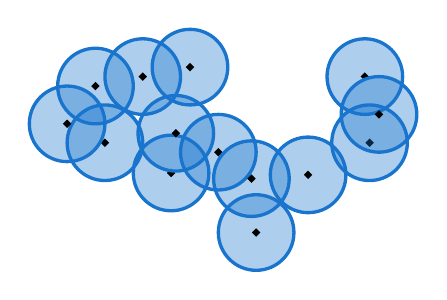
\begin{tikzpicture}[scale=1.2]
			% \draw[help lines] (-1,-1) grid (2,2);
			\coordinate (1) at (0,-0.02);
			\coordinate (2) at (.05,.4);
			\coordinate (3) at (.5,.2);
			\coordinate (4) at (.85,-.08);
			\coordinate (5) at (1.45,-.04);
			\coordinate (6) at (-0.7,.3);
			\coordinate (7) at (2.1,.3);
			\coordinate (8) at (2.05,1);
			\coordinate (9) at (0.2,1.1);
			\coordinate (10) at (.9,-.65);
			\coordinate (11) at (2.2,.6);
			\coordinate (12) at (-.3,1);
			\coordinate (13) at (-.8,.9);
			\coordinate (14) at (-1.1,.5);
			\foreach \x in {1,2,...,14}{
				\draw[DodgerBlue3,fill=DodgerBlue3,fill opacity=.35,very thick] (\x) circle[radius=.4];
				\draw[fill,very thick] (\x) circle[radius=.02];
			}
		\end{tikzpicture}
	}
	\hspace{2cm}
	\subfloat[Mit $\varepsilon=\SI{0.3}{\centi\metre}$ erhält man drei Komponenten]{
		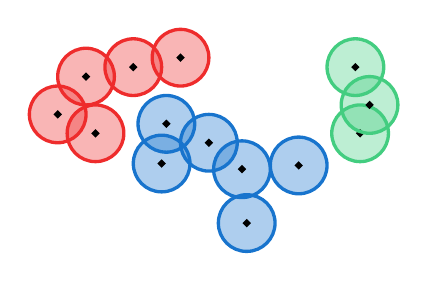
\begin{tikzpicture}[scale=1.2]
			% \draw[help lines] (-1,-1) grid (2,2);
			\coordinate (1) at (0,-0.02);
			\coordinate (2) at (.05,.4);
			\coordinate (3) at (.5,.2);
			\coordinate (4) at (.85,-.08);
			\coordinate (5) at (1.45,-.04);
			\coordinate (6) at (-0.7,.3);
			\coordinate (7) at (2.1,.3);
			\coordinate (8) at (2.05,1);
			\coordinate (9) at (0.2,1.1);
			\coordinate (10) at (.9,-.65);
			\coordinate (11) at (2.2,.6);
			\coordinate (12) at (-.3,1);
			\coordinate (13) at (-.8,.9);
			\coordinate (14) at (-1.1,.5);
			\foreach \x in {1,2,...,5,10}{
				\draw[DodgerBlue3,fill=DodgerBlue3,fill opacity=.35,very thick] (\x) circle[radius=.3];
				\draw[fill,very thick] (\x) circle[radius=.02];
			}
			\foreach \x in {6,9,12,13,14}{
				\draw[Firebrick2,fill=Firebrick2,fill opacity=.35,very thick] (\x) circle[radius=.3];
				\draw[fill,very thick] (\x) circle[radius=.02];
			}
			\foreach \x in {7,8,11}{
				\draw[SeaGreen3,fill=SeaGreen3,fill opacity=.35,very thick] (\x) circle[radius=.3];
				\draw[fill,very thick] (\x) circle[radius=.02];
			}
		\end{tikzpicture}
	}
	\caption{Komponenten einer 14-elementigen Punktmenge zu verschiedenen $\varepsilon$-Werten}\label{fig:components}
\end{figure}

\begin{definition}[{name=[Gruppe während eines Zeitraums]}]
	Eine Menge $G$ von $k$ Entitäten bildet eine \Index{Gruppe} im Zeitintervall $I$, falls folgendes gilt:
	\begin{enumerate}[(i)]
		\item $G$ enthält mindestens $m$ Entitäten, also $k \ge m$
		\item die Länge von $I$ ist mindestens $\delta$
		\item zu jeder Zeit $t \in I$ existiert eine Komponente $C \in \mathcal{C}(t)$ mit $G \subseteq C$.
	\end{enumerate}
	Das Intervall $I=[t_s,t_e]$ der Gruppe $G$ bezeichnen wir auch mit $I_G$.
	Eine Gruppe $H$ \bet{überlagert}\index{Gruppe!überlagernde} $G$, falls $G \subseteq H$ und $I_G \subseteq I_H$ gilt.
	Falls kein solches $H$ existiert, so heißt $G$ \bet{maximal}\index{Gruppe!maximale}. 
\end{definition}

Da wir ja eigentlich die Trajektorien einzelner Entitäten gruppieren wollen, mag es auf den ersten Blick etwas kontraintuitiv erscheinen, dass eine Entität $x$ in mehreren maximalen Gruppen enthalten sein kann, da zum Überlagern auch die Inklusion der Zeitintervalle gegeben sein muss.

% chapter def_gruppe (end)






\cleardoubleoddemptypage
\pagenumbering{Alph}
\setcounter{page}{1}
\appendix
\printbibliography
\printindex
\todototoc
\listoftodos[To-do's und andere Baustellen]
\end{document}